\chapter{The Two Prisoners}

A year after Louis XVIII.’s restoration, a visit was made by the
inspector-general of prisons. Dantès in his cell heard the noise of
preparation,—sounds that at the depth where he lay would have been
inaudible to any but the ear of a prisoner, who could hear the splash
of the drop of water that every hour fell from the roof of his dungeon.
He guessed something uncommon was passing among the living; but he had
so long ceased to have any intercourse with the world, that he looked
upon himself as dead.

The inspector visited, one after another, the cells and dungeons of
several of the prisoners, whose good behavior or stupidity recommended
them to the clemency of the government. He inquired how they were fed,
and if they had any request to make. The universal response was, that
the fare was detestable, and that they wanted to be set free.

The inspector asked if they had anything else to ask for. They shook
their heads. What could they desire beyond their liberty? The inspector
turned smilingly to the governor.

“I do not know what reason government can assign for these useless
visits; when you see one prisoner, you see all,—always the same
thing,—ill fed and innocent. Are there any others?”

“Yes; the dangerous and mad prisoners are in the dungeons.”

“Let us visit them,” said the inspector with an air of fatigue. “We
must play the farce to the end. Let us see the dungeons.”

“Let us first send for two soldiers,” said the governor. “The prisoners
sometimes, through mere uneasiness of life, and in order to be
sentenced to death, commit acts of useless violence, and you might fall
a victim.”

“Take all needful precautions,” replied the inspector.

Two soldiers were accordingly sent for, and the inspector descended a
stairway, so foul, so humid, so dark, as to be loathsome to sight,
smell, and respiration.

“Oh,” cried the inspector, “who can live here?”

“A most dangerous conspirator, a man we are ordered to keep the most
strict watch over, as he is daring and resolute.”

“He is alone?”

“Certainly.”

“How long has he been there?”

“Nearly a year.”

“Was he placed here when he first arrived?”

“No; not until he attempted to kill the turnkey, who took his food to
him.”

“To kill the turnkey?”

“Yes, the very one who is lighting us. Is it not true, Antoine?” asked
the governor.

“True enough; he wanted to kill me!” returned the turnkey.

“He must be mad,” said the inspector.

“He is worse than that,—he is a devil!” returned the turnkey.

“Shall I complain of him?” demanded the inspector.

“Oh, no; it is useless. Besides, he is almost mad now, and in another
year he will be quite so.”

“So much the better for him,—he will suffer less,” said the inspector.
He was, as this remark shows, a man full of philanthropy, and in every
way fit for his office.

“You are right, sir,” replied the governor; “and this remark proves
that you have deeply considered the subject. Now we have in a dungeon
about twenty feet distant, and to which you descend by another stair,
an old abbé, formerly leader of a party in Italy, who has been here
since 1811, and in 1813 he went mad, and the change is astonishing. He
used to weep, he now laughs; he grew thin, he now grows fat. You had
better see him, for his madness is amusing.”

“I will see them both,” returned the inspector; “I must conscientiously
perform my duty.”

This was the inspector’s first visit; he wished to display his
authority.

“Let us visit this one first,” added he.

“By all means,” replied the governor, and he signed to the turnkey to
open the door. At the sound of the key turning in the lock, and the
creaking of the hinges, Dantès, who was crouched in a corner of the
dungeon, whence he could see the ray of light that came through a
narrow iron grating above, raised his head. Seeing a stranger, escorted
by two turnkeys holding torches and accompanied by two soldiers, and to
whom the governor spoke bareheaded, Dantès, who guessed the truth, and
that the moment to address himself to the superior authorities was
come, sprang forward with clasped hands.

The soldiers interposed their bayonets, for they thought that he was
about to attack the inspector, and the latter recoiled two or three
steps. Dantès saw that he was looked upon as dangerous. Then, infusing
all the humility he possessed into his eyes and voice, he addressed the
inspector, and sought to inspire him with pity.

The inspector listened attentively; then, turning to the governor,
observed, “He will become religious—he is already more gentle; he is
afraid, and retreated before the bayonets—madmen are not afraid of
anything; I made some curious observations on this at Charenton.” Then,
turning to the prisoner, “What is it you want?” said he.

“I want to know what crime I have committed—to be tried; and if I am
guilty, to be shot; if innocent, to be set at liberty.”

“Are you well fed?” said the inspector.

“I believe so; I don’t know; it’s of no consequence. What matters
really, not only to me, but to officers of justice and the king, is
that an innocent man should languish in prison, the victim of an
infamous denunciation, to die here cursing his executioners.”

“You are very humble today,” remarked the governor; “you are not so
always; the other day, for instance, when you tried to kill the
turnkey.”

“It is true, sir, and I beg his pardon, for he has always been very
good to me, but I was mad.”

“And you are not so any longer?”

“No; captivity has subdued me—I have been here so long.”

“So long?—when were you arrested, then?” asked the inspector.

“The 28th of February, 1815, at half-past two in the afternoon.”

“Today is the 30th of July, 1816,—why, it is but seventeen months.”

“Only seventeen months,” replied Dantès. “Oh, you do not know what is
seventeen months in prison!—seventeen ages rather, especially to a man
who, like me, had arrived at the summit of his ambition—to a man, who,
like me, was on the point of marrying a woman he adored, who saw an
honorable career opened before him, and who loses all in an instant—who
sees his prospects destroyed, and is ignorant of the fate of his
affianced wife, and whether his aged father be still living! Seventeen
months’ captivity to a sailor accustomed to the boundless ocean, is a
worse punishment than human crime ever merited. Have pity on me, then,
and ask for me, not intelligence, but a trial; not pardon, but a
verdict—a trial, sir, I ask only for a trial; that, surely, cannot be
denied to one who is accused!”

“We shall see,” said the inspector; then, turning to the governor, “On
my word, the poor devil touches me. You must show me the proofs against
him.”

“Certainly; but you will find terrible charges.”

“Monsieur,” continued Dantès, “I know it is not in your power to
release me; but you can plead for me—you can have me tried—and that is
all I ask. Let me know my crime, and the reason why I was condemned.
Uncertainty is worse than all.”

“Go on with the lights,” said the inspector.

“Monsieur,” cried Dantès, “I can tell by your voice you are touched
with pity; tell me at least to hope.”

“I cannot tell you that,” replied the inspector; “I can only promise to
examine into your case.”

“Oh, I am free—then I am saved!”

“Who arrested you?”

“M. Villefort. See him, and hear what he says.”

“M. Villefort is no longer at Marseilles; he is now at Toulouse.”

“I am no longer surprised at my detention,” murmured Dantès, “since my
only protector is removed.”

“Had M. de Villefort any cause of personal dislike to you?”

“None; on the contrary, he was very kind to me.”

“I can, then, rely on the notes he has left concerning you?”

“Entirely.”

“That is well; wait patiently, then.”

Dantès fell on his knees, and prayed earnestly. The door closed; but
this time a fresh inmate was left with Dantès—Hope.

\begin{figure}[h]
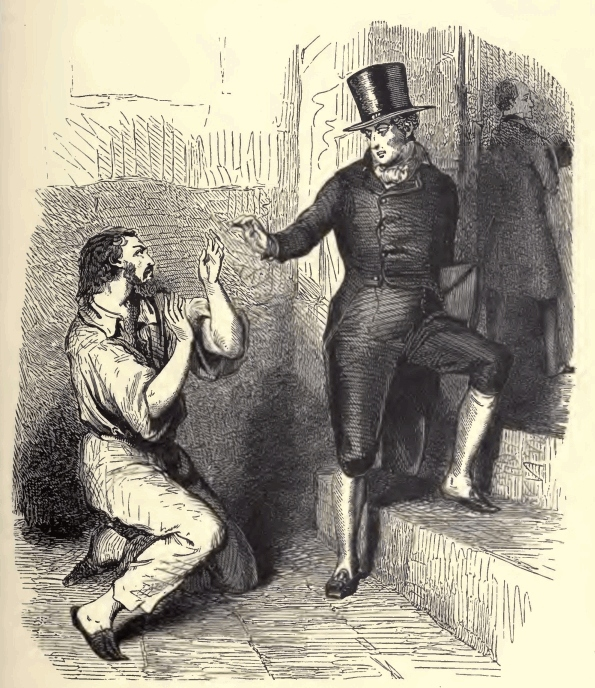
\includegraphics[width=\textwidth]{0173m.jpg}
\end{figure}

“Will you see the register at once,” asked the governor, “or proceed to
the other cell?”

“Let us visit them all,” said the inspector. “If I once went up those
stairs. I should never have the courage to come down again.”

“Ah, this one is not like the other, and his madness is less affecting
than this one’s display of reason.”

“What is his folly?”

“He fancies he possesses an immense treasure. The first year he offered
government a million of francs for his release; the second, two; the
third, three; and so on progressively. He is now in his fifth year of
captivity; he will ask to speak to you in private, and offer you five
millions.”

“How curious!—what is his name?”

“The Abbé Faria.”

“No. 27,” said the inspector.

“It is here; unlock the door, Antoine.”

The turnkey obeyed, and the inspector gazed curiously into the chamber
of the \textit{mad abbé}, as the prisoner was usually called.

In the centre of the cell, in a circle traced with a fragment of
plaster detached from the wall, sat a man whose tattered garments
scarcely covered him. He was drawing in this circle geometrical lines,
and seemed as much absorbed in his problem as Archimedes was when the
soldier of Marcellus slew him. He did not move at the sound of the
door, and continued his calculations until the flash of the torches
lighted up with an unwonted glare the sombre walls of his cell; then,
raising his head, he perceived with astonishment the number of persons
present. He hastily seized the coverlet of his bed, and wrapped it
round him.

“What is it you want?” said the inspector.

“I, monsieur,” replied the abbé with an air of surprise,—“I want
nothing.”

“You do not understand,” continued the inspector; “I am sent here by
government to visit the prison, and hear the requests of the
prisoners.”

“Oh, that is different,” cried the abbé; “and we shall understand each
other, I hope.”

“There, now,” whispered the governor, “it is just as I told you.”

“Monsieur,” continued the prisoner, “I am the Abbé Faria, born at Rome.
I was for twenty years Cardinal Spada’s secretary; I was arrested, why,
I know not, toward the beginning of the year 1811; since then I have
demanded my liberty from the Italian and French government.”

“Why from the French government?”

“Because I was arrested at Piombino, and I presume that, like Milan and
Florence, Piombino has become the capital of some French department.”

“Ah,” said the inspector, “you have not the latest news from Italy?”

“My information dates from the day on which I was arrested,” returned
the Abbé Faria; “and as the emperor had created the kingdom of Rome for
his infant son, I presume that he has realized the dream of Machiavelli
and Cæsar Borgia, which was to make Italy a united kingdom.”

“Monsieur,” returned the inspector, “Providence has changed this
gigantic plan you advocate so warmly.”

“It is the only means of rendering Italy strong, happy, and
independent.”

“Very possibly; only I am not come to discuss politics, but to inquire
if you have anything to ask or to complain of.”

“The food is the same as in other prisons,—that is, very bad; the
lodging is very unhealthful, but, on the whole, passable for a dungeon;
but it is not that which I wish to speak of, but a secret I have to
reveal of the greatest importance.”

“We are coming to the point,” whispered the governor.

“It is for that reason I am delighted to see you,” continued the abbé,
“although you have disturbed me in a most important calculation, which,
if it succeeded, would possibly change Newton’s system. Could you allow
me a few words in private.”

“What did I tell you?” said the governor.

“You knew him,” returned the inspector with a smile.

“What you ask is impossible, monsieur,” continued he, addressing Faria.

\begin{figure}[ht]
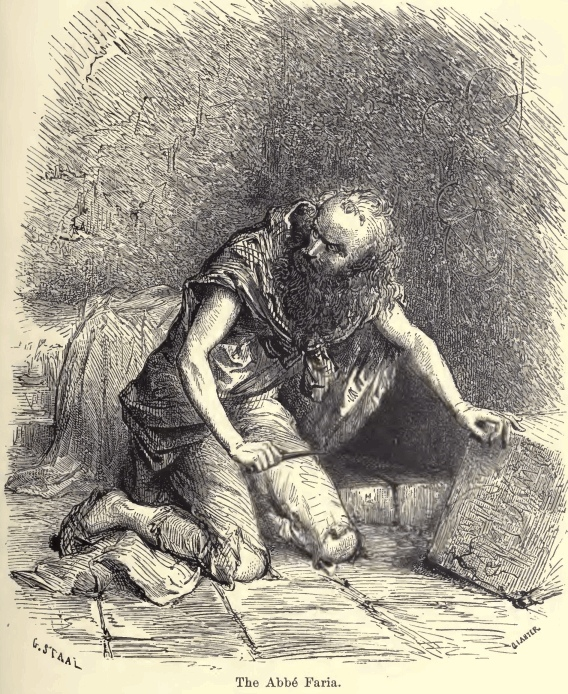
\includegraphics[width=\textwidth]{0175m.jpg}
\end{figure}

“But,” said the abbé, “I would speak to you of a large sum, amounting
to five millions.”

“The very sum you named,” whispered the inspector in his turn.

“However,” continued Faria, seeing that the inspector was about to
depart, “it is not absolutely necessary for us to be alone; the
governor can be present.”

“Unfortunately,” said the governor, “I know beforehand what you are
about to say; it concerns your treasures, does it not?” Faria fixed his
eyes on him with an expression that would have convinced anyone else of
his sanity.

“Of course,” said he; “of what else should I speak?”

“Mr. Inspector,” continued the governor, “I can tell you the story as
well as he, for it has been dinned in my ears for the last four or five
years.”

“That proves,” returned the abbé, “that you are like those of Holy
Writ, who having eyes see not, and having ears hear not.”

“My dear sir, the government is rich and does not want your treasures,”
replied the inspector; “keep them until you are liberated.” The abbé’s
eyes glistened; he seized the inspector’s hand.

“But what if I am not liberated,” cried he, “and am detained here until
my death? this treasure will be lost. Had not government better profit
by it? I will offer six millions, and I will content myself with the
rest, if they will only give me my liberty.”

“On my word,” said the inspector in a low tone, “had I not been told
beforehand that this man was mad, I should believe what he says.”

“I am not mad,” replied Faria, with that acuteness of hearing peculiar
to prisoners. “The treasure I speak of really exists, and I offer to
sign an agreement with you, in which I promise to lead you to the spot
where you shall dig; and if I deceive you, bring me here again,—I ask
no more.”

The governor laughed. “Is the spot far from here?”

“A hundred leagues.”

“It is not ill-planned,” said the governor. “If all the prisoners took
it into their heads to travel a hundred leagues, and their guardians
consented to accompany them, they would have a capital chance of
escaping.”

“The scheme is well known,” said the inspector; “and the abbé’s plan
has not even the merit of originality.”

Then turning to Faria, “I inquired if you are well fed?” said he.

“Swear to me,” replied Faria, “to free me if what I tell you prove
true, and I will stay here while you go to the spot.”

“Are you well fed?” repeated the inspector.

“Monsieur, you run no risk, for, as I told you, I will stay here; so
there is no chance of my escaping.”

“You do not reply to my question,” replied the inspector impatiently.

“Nor you to mine,” cried the abbé. “You will not accept my gold; I will
keep it for myself. You refuse me my liberty; God will give it me.” And
the abbé, casting away his coverlet, resumed his place, and continued
his calculations.

\begin{figure}[ht]
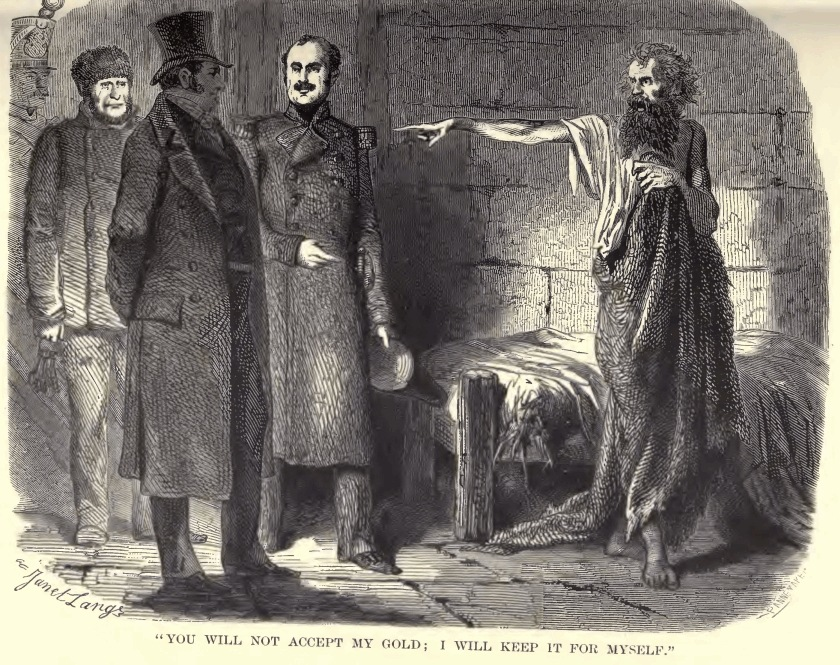
\includegraphics[width=\textwidth]{0177m.jpg}
\end{figure}

“What is he doing there?” said the inspector.

“Counting his treasures,” replied the governor.

Faria replied to this sarcasm with a glance of profound contempt. They
went out. The turnkey closed the door behind them.

“He was wealthy once, perhaps?” said the inspector.

“Or dreamed he was, and awoke mad.”

“After all,” said the inspector, “if he had been rich, he would not
have been here.”

So the matter ended for the Abbé Faria. He remained in his cell, and
this visit only increased the belief in his insanity.

Caligula or Nero, those treasure-seekers, those desirers of the
impossible, would have accorded to the poor wretch, in exchange for his
wealth, the liberty he so earnestly prayed for. But the kings of modern
times, restrained by the limits of mere probability, have neither
courage nor desire. They fear the ear that hears their orders, and the
eye that scrutinizes their actions. Formerly they believed themselves
sprung from Jupiter, and shielded by their birth; but nowadays they are
not inviolable.

It has always been against the policy of despotic governments to suffer
the victims of their persecutions to reappear. As the Inquisition
rarely allowed its victims to be seen with their limbs distorted and
their flesh lacerated by torture, so madness is always concealed in its
cell, from whence, should it depart, it is conveyed to some gloomy
hospital, where the doctor has no thought for man or mind in the
mutilated being the jailer delivers to him. The very madness of the
Abbé Faria, gone mad in prison, condemned him to perpetual captivity.

The inspector kept his word with Dantès; he examined the register, and
found the following note concerning him:

\textit{Edmond Dantès:}

Violent Bonapartist; took an active part in the return from Elba.

The greatest watchfulness and care to be exercised.

This note was in a different hand from the rest, which showed that it
had been added since his confinement. The inspector could not contend
against this accusation; he simply wrote, \textit{Nothing to be done.}

This visit had infused new vigor into Dantès; he had, till then,
forgotten the date; but now, with a fragment of plaster, he wrote the
date, 30th July, 1816, and made a mark every day, in order not to lose
his reckoning again. Days and weeks passed away, then months—Dantès
still waited; he at first expected to be freed in a fortnight. This
fortnight expired, he decided that the inspector would do nothing until
his return to Paris, and that he would not reach there until his
circuit was finished, he therefore fixed three months; three months
passed away, then six more. Finally ten months and a half had gone by
and no favorable change had taken place, and Dantès began to fancy the
inspector’s visit but a dream, an illusion of the brain.

At the expiration of a year the governor was transferred; he had
obtained charge of the fortress at Ham. He took with him several of his
subordinates, and amongst them Dantès’ jailer. A new governor arrived;
it would have been too tedious to acquire the names of the prisoners;
he learned their numbers instead. This horrible place contained fifty
cells; their inhabitants were designated by the numbers of their cell,
and the unhappy young man was no longer called Edmond Dantès—he was now
number 34.
